\documentclass[12pt,a4paper]{article}
\usepackage[utf8]{inputenc}
\usepackage{amsmath}
\usepackage{amsfonts}
\usepackage{amssymb}
%\usepackage{tikz}
\usepackage{graphicx}
%\usetikzlibrary{positioning}
\usepackage{tabularx}

%\usepackage{algorithm}
%\usepackage[noend]{algpseudocode}
%\def\BState{\State\hskip-\ALG@thistlm}

\usepackage{hyperref}
\usepackage{color}
\hypersetup{
	colorlinks,
	filecolor=black,
	linkcolor=black,
	urlcolor=black
}
\usepackage{listings}
\usepackage{xcolor}
\definecolor{codegreen}{rgb}{0,0.6,0}
\definecolor{codegray}{rgb}{0.5,0.5,0.5}
\definecolor{codepurple}{rgb}{0.58,0,0.82}
\definecolor{backcolour}{rgb}{0.95,0.95,0.92}

\lstdefinestyle{codestyle}{
    backgroundcolor=\color{backcolour},   
    commentstyle=\color{codegreen},
    keywordstyle=\color{magenta},
    numberstyle=\tiny\color{codegray},
    stringstyle=\color{codepurple},
    basicstyle=\ttfamily\footnotesize,
    breakatwhitespace=false,         
    breaklines=true,                 
    captionpos=b,                    
    keepspaces=true,                 
    numbers=left,                    
    numbersep=5pt,                  
    showspaces=false,                
    showstringspaces=false,
    showtabs=false,                  
    tabsize=2
}
\lstset{style=codestyle}

\setlength{\parindent}{0cm}
\UseRawInputEncoding
\newcommand{\listedsection}[1]{\section*{#1}\addcontentsline{toc}{section}{#1}}
\newcommand{\listedsubsection}[1]{\subsection*{#1}\addcontentsline{toc}{subsection}{#1}}

\author{David Bohner 18-951-822, Romeo Stoll 19-917-749}
\title{WNMC: Exercise 05 - VLC}
\date{Fall 2021}


\begin{document}
\maketitle
\tableofcontents
\newpage

\listedsection{Step 2}
\listedsubsection{Answers}
\begin{itemize}
\item[1.] \textbf{What is the bandwidth of the optical spectrum?}
\item[] The frequency range of visible light lies at around 430 - 750 THz. [1] This constitutes a band 320 THz in size, which by Prof. Mangold's bandwidth estimation guidelines corresponds to 320 Tb/s.
\item[2.] \textbf{Is the visible spectrum regulated?}
\item[] No.
\item[3.] \textbf{What is the difference between infrared and visible light?}
\item[] Infrared light is light at a frequency lower than the lowest frequency visible to the human eye. (This also implies a lower energy of the wave.)
\item[4.] \textbf{Can infrared light penetrate water? Can visible light?}
\item[] Infrared light \textit{can} penetrate water for a limited range, however water \textit{does} have IR-absorbing properties, making it inefficient/ineffective at long-range underwater communication. Higher-power visible light, such as blue or violet light, is less-absorbed and as such a better frequency to communicate underwater with.
\item[5.] \textbf{How do submarines communicate through the ocean, when they operate below water surface?}
\item[] Sound waves, microwaves, blue LED/lasers (i.e. high-energy visible light). (Lecture 06: VLC)
\item[6.] \textbf{How can an LED be used as a receiver?}
\item[] LEDs lose charge more quickly while in contact with photons. This allows for charge depletion rate comparisons to detect if another LED was lit up (e.g. transmitting a 1-bit, depending on implementation) or not.
\item[7.] \textbf{What are the benefits of using an LED instead of a photodiode as a receiver in consumer electronics?}
\item[] Price/practicality. Installing both an LED and a photodiode for two-way communication would be both more expensive (added product) as well as more challenging to implement. (Design: only need to place 1 LED instead of both components. Hardware: Photodiode may require a more complicated microcontroller. Price: Beyond additional design costs, the hardware of the photodiode itself obviously adds to manufacturing cost.)
\item[] Additionally, many consumer electronics already contain some kind of LED, allowing for communication implementation by just changing microcontroller programming rather than re-designing hardware.
\item[]
\item[{[1]}] https://www.britannica.com/science/color/The-visible-spectrum
\end{itemize}

\listedsection{Step 3}

\listedsection{Step 4}
\listedsubsection{Screenshots}
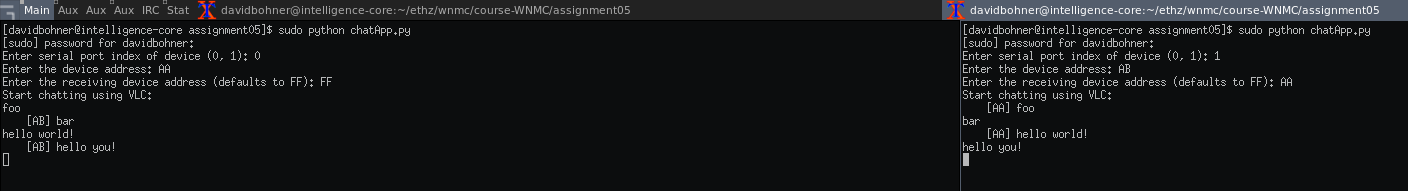
\includegraphics[width=\linewidth]{chatApp communication.png} 
\listedsection{Step 5}
\listedsubsection{Throughput, Delay Plots}
\listedsubsection{Interpretation}

\newpage
\listedsection{Appendix}
\listedsubsection{Step 4: Chat App Source Code}
\lstinputlisting[language=Python]{chatApp.py}
\newpage

\listedsubsection{Step 5: Script}
\lstinputlisting[language=Python]{distanceMeasurement.py}
\end{document}